\documentclass{article}
\usepackage[T1]{fontenc}
\usepackage[utf8]{inputenc}
\usepackage{lmodern}
\usepackage[ngerman]{babel}
\usepackage{amsmath, amssymb}
\usepackage{array}
%\usepackage{memoir}
\usepackage{phonetic} % for reversed D
\usepackage{wasysym}  % for the notes
\usepackage{tikz, tikzsymbols}
\usepackage{xcolor}
\usetikzlibrary{arrows,automata,fit}
\setlength\parindent{0pt}

    
\begin{document}

\begin{center}
  \Large{Informatik \revD: Übungsblatt 7}

  \large{Sebastian Höffner, Andrea Suckro}
\end{center}



\section*{Aufgabe 7.1}
Gegeben sei: $L=\{d^ja^kb^lc^m | (j=0) oder (k=l=m) \}$
\subsection*{a)}
Intuitiv scheint die Sprache L nicht kontextfrei zu sein, da sie als Teilsprache $L_1=\{d^ja^ib^ic^i | j > 0 \}$ enthält und wir mit Hilfe eines Homomorphismus ($d=\epsilon$) auf $L'=\{a^ib^ic^i\}$ kommen können und aus der Vorlesung wissen, dass diese nicht kontextfrei ist.
\subsection*{b)}
Wir können nun quasi zwei Fälle betrachten. Erinnerung Regeln für das Pumping Lemma:
\begin{align*}
z &= uvwxy \\
|vx| &\geq 1\\
|vwx| &\leq n \\
\forall i &\geq 0: uv^iwx^iy\in L 
\end{align*}
\subsubsection*{1.Fall $j=0$}
In diesem Fall bekommen wir die Sprache $L'=\{a^kb^lc^m\}$.Nun versuchen wir darauf das Pumping Lemma anzuwenden. Dazu wählen wir für ein beliebiges Wort $z\in L',|z|\geq n$ (n ist die Mindestwortlänge) folgende Zerlegung: $v\in \{a,b,c\}$, abhängig davon dass der Buchstabe in dem Wort das wir gerade betrachten vorkommt. $x$ lassen wir komplett leer. Damit ist $|vx| \geq 1$ erfüllt. $w$ können wir ebenfalls leer lassen. Damit ist auch $|vwx| \leq n$ erfüllt. In $u$ und $y$ packen wir den Rest des Wortes. Wenn wir nun $v$ aufpumpen vergrößern wir $k | l | m$ und landen damit wieder $\in L'$. Das Pumping Lemma ist also für diesen Fall erfüllt.
\subsubsection*{2.Fall $k=l=m$}
In diesem Fall haben wir wieder zwei Fälle. Einmal ist $j=0$, damit landen wir aber im ersten Fall (genauer gesagt ist dann $\{a^kb^kc^k\} \subset \{a^kb^lc^m\}$). Im zweiten Fall ist $j>0$. Wir betrachten also $L'=\{d^ja^ib^ic^i|j>0\}$. Als Zerlegung können wir nun $u$,$x$ und $w$ wieder leer wählen und $v=d^j, |j|\leq n$ (das bedeutet, dass nicht alle d's in $v$ enthalten sein müssen). $|vx| \geq 1$ und $|vwx| \leq n$ sind somit erfüllt. Wenn wir nun $v$ aufpumpen bekommen wir nur d's hinzu und erhalten so wieder ein Wort $\in L$.


\section*{Aufgabe 7.2}



\section*{Aufgabe 7.3}
\subsection*{Leerheitsproblem}
\begin{center}
Initial:\\
\begin{tabular}{ll}
$S \rightarrow E | ABC$               & $A \rightarrow bDC | E | S$ \\
$B \rightarrow acDC | C$              & $C \rightarrow ab | Ja | IdA$ \\
$D \rightarrow deF | DeF | dEF | DEF$ & $E \rightarrow abba | aBBa | AbbA$ \\
$F \rightarrow JcJ | GJ | bG$         & $G \rightarrow F | IG$ \\
$H \rightarrow SA | Hcc$              & $I \rightarrow c | cIc | dF$
\end{tabular}\\
Erster Schritt:\\
\begin{tabular}{ll}
$S \rightarrow {\color{red}E} | AB{\color{red}C}$               & $A \rightarrow bD{\color{red}C} | {\color{red}E} | S$ \\
$B \rightarrow acD{\color{red}C} | {\color{red}C}$              & ${\color{red}C} \rightarrow ab | Ja | {\color{red}I}dA$ \\
$D \rightarrow deF | DeF | d{\color{red}E}F | D{\color{red}E}F$ & ${\color{red}E} \rightarrow abba | aBBa | AbbA$ \\
$F \rightarrow JcJ | GJ | bG$                                   & $G \rightarrow F | {\color{red}I}G$ \\
$H \rightarrow SA | Hcc$                                        & ${\color{red}I} \rightarrow c | c{\color{red}I}c | dF$
\end{tabular}\\
Zweiter Schritt:\\
\begin{tabular}{ll}
${\color{red}S} \rightarrow {\color{red}E} | {\color{red}ABC}$  & ${\color{red}A} \rightarrow bD{\color{red}C} | {\color{red}E} | {\color{red}S}$ \\
${\color{red}B} \rightarrow acD{\color{red}C} | {\color{red}C}$ & ${\color{red}C} \rightarrow ab | Ja | {\color{red}I}d{\color{red}A}$ \\
$D \rightarrow deF | DeF | d{\color{red}E}F | D{\color{red}E}F$ & ${\color{red}E} \rightarrow abba | a{\color{red}BB}a | {\color{red}A}bb{\color{red}A}$ \\
$F \rightarrow JcJ | GJ | bG$                                   & $G \rightarrow F | {\color{red}I}G$ \\
$H \rightarrow {\color{red}SA} | Hcc$                           & ${\color{red}I} \rightarrow c | c{\color{red}I}c | dF$
\end{tabular}
\end{center}
Bereits im zweiten Schritt wird $S$ markiert, also ist $L(G) \neq \emptyset$.

\subsection*{Endlichkeitsproblem}
Wir führen den Algorithmus von oben vorerst zu Ende.
\begin{center}
Dritter Schritt:\\
\begin{tabular}{ll}
${\color{red}S} \rightarrow {\color{red}E} | {\color{red}ABC}$  & ${\color{red}A} \rightarrow bD{\color{red}C} | {\color{red}E} | {\color{red}S}$ \\
${\color{red}B} \rightarrow acD{\color{red}C} | {\color{red}C}$ & ${\color{red}C} \rightarrow ab | Ja | {\color{red}I}d{\color{red}A}$ \\
$D \rightarrow deF | DeF | d{\color{red}E}F | D{\color{red}E}F$ & ${\color{red}E} \rightarrow abba | a{\color{red}BB}a | {\color{red}A}bb{\color{red}A}$ \\
$F \rightarrow JcJ | GJ | bG$                                   & $G \rightarrow F | {\color{red}I}G$ \\
${\color{red}H} \rightarrow {\color{red}SA} | {\color{red}H}cc$ & ${\color{red}I} \rightarrow c | c{\color{red}I}c | dF$
\end{tabular}
\end{center}
Weiter lässt sich nichts markieren, d.h. wir können die Grammatik nun auf die markierten Regeln reduzieren.
\begin{center}
\begin{tabular}{ll}
$S \rightarrow E | ABC$            & $A \rightarrow E | S$ \\
$B \rightarrow C$                  & $C \rightarrow ab | IdA$ \\
$E \rightarrow abba | aBBa | AbbA$ & $H \rightarrow SA | Hcc$ \\
$I \rightarrow c | cIc$            & \\
\end{tabular}
\end{center}
Als nächstes reduzieren wir die Grammatik auf erreichbare Regeln.
\begin{center}
\begin{tabular}{ll}
${\color{red}S} \rightarrow {\color{red}E} | {\color{red}ABC}$                         & ${\color{red}A} \rightarrow {\color{red}E} | {\color{red}S}$ \\
${\color{red}B} \rightarrow {\color{red}C}$                                            & ${\color{red}C} \rightarrow ab | {\color{red}I}d{\color{red}A}$ \\
${\color{red}E} \rightarrow abba | a{\color{red}BB}a | {\color{red}A}bb{\color{red}A}$ & $H \rightarrow SA | Hcc$ \\
${\color{red}I} \rightarrow c | c{\color{red}I}c$                                      & \\
\end{tabular}
\end{center}
Übrig bleiben:
\begin{center}
\begin{tabular}{ll}
$S \rightarrow E | ABC$            & $A \rightarrow E | S$ \\
$B \rightarrow C$                  & $C \rightarrow ab | IdA$ \\
$E \rightarrow abba | aBBa | AbbA$ & $I \rightarrow c | cIc$ \\
\end{tabular}
\end{center}
Die Regeln $S \rightarrow E$, $A \rightarrow E$, $A \rightarrow S$ und $B \rightarrow C$ müssen transformiert werden. Die transformierte Grammatik sieht z.B. so aus:
\begin{center}
\begin{tabular}{ll}
$S \rightarrow abba | aBBa | AbbA | ABC$ & $A \rightarrow abba | aBBa | AbbA | ABC$ \\
$B \rightarrow ab | IdA$                 & $C \rightarrow ab | IdA$ \\
$E \rightarrow abba | AbbA | aBBa$       & $I \rightarrow c | cIc$ \\
\end{tabular}
\end{center}

Wir erstellen einen Hilfsgraph auf Grundlage der reduzierten und vereinfachten Grammatik.
\begin{center}
\begin{tikzpicture}[->, auto, node distance=2cm]
  \node[state] (S)                   {$S$};
  \node[state] (A) [right of=S]      {$A$};
  \node[state] (B) [below of=S]      {$B$};
  \node[state] (C) [above of=S] {$C$};
  \node[state] (E) [right of=B]      {$E$}; 
  \node[state] (I) [left of=S] {$I$};

  \path (S) edge node {} (A)
            edge node {} (B)
            edge node {} (C)
        (A) edge [bend left] node {} (B)
            edge [bend left] node {} (C)
            edge [loop right] node {} (A)
        (B) edge [bend left] node {} (A)
            edge node {} (I)
        (C) edge [bend left] node {} (A)
            edge node {} (I)
        (E) edge node {} (A)
            edge node {} (B)
        (I) edge [loop below] node {} (I)    
        ;
\end{tikzpicture}
\end{center}

Es gibt gerichtete Kreise $B \leftrightarrow A \leftrightarrow C$, sowie $A$ und $I$ auf sich selbst. Somit ist $|L(G)| = \infty$.



\section*{Aufgabe 7.4}
Zur besseren Lesbarkeit wird folgende Bennenung der Elemente der Definition vorgenommen:
\begin{align*}
uUw \rightarrow uyw && U \in V, u,w,y \in \left( V \cup \Sigma \right)^* && |y| \geq 1
\end{align*}

Die Regel $AB\rightarrow BA$ ist nach der neuen Definition nicht erlaubt, da $U \in V$ gegeben ist, somit entweder $A$ oder $B$ der linken Seite das $U \in V$ repräsentiert. Dadurch ergeben sich zwei Fälle:
\begin{itemize}
	\item $U = A$: In diesem Fall wäre auf der linken Seite $w = B$, wodurch aber die Bedingung $uyw$ nicht erfüllt werden kann, da nach $w$ keine Symbole mehr kommen dürfen - in $BA$ wäre das jedoch der Fall.
  \item $U = B$: In diesem Fall ist es umgekehrt: $u = A$, wodurch ebenfalls $uyw$ nicht erfüllt werden kann. Vor $u$ dürfen keine Symbole auftreten, was bei $BA$ jedoch der Fall wäre.
\end{itemize}

\subsection*{Algorithmus}
Um die Regel $AB \rightarrow BA$ von der alten in die neue Definition zu überführen, geht man wie folgt vor:

\begin{enumerate}
	\item Erstelle Regeln mit neuen Variablen um beide Seiten darzustellen.\\ $AB \rightarrow BA \Rightarrow X \rightarrow AB, Y \rightarrow BA$
  \item Füge Regel $X \rightarrow Y$ in die Grammatik ein und entferne problematische Regel.
\end{enumerate}

\subsection*{Konkrekter Fall}
\begin{align*}
\begin{array}{l|l|l}
\text{Initial}    & \text{Schritt 1}  & \text{Schritt 2} \\ \hline
AB \rightarrow BA & AB \rightarrow BA & X \rightarrow Y  \\
                  & X  \rightarrow AB & X \rightarrow AB \\
                  & Y  \rightarrow BA & Y \rightarrow BA \\
\end{array}
\end{align*}

\subsection*{Erläuterung}
Im Algorithmus sind die Regeln $X \rightarrow AB$ bzw. $Y \rightarrow BA$ in der gegebenen Form, da $X$ bzw. $Y$ Elemente in $V$ sind, $u$ und $w$ leer sind (nach Definition erlaubt) und $y=AB$ bzw. $y=BA$ und damit auch $|y|\geq$ sowie alle weiteren Bedingungen erfüllt sind.

Die Regel $X \rightarrow Y$ funktioniert ebenfalls nach dem selben Prinzip.


\section*{Aufgabe 7.5}
\begin{figure}[ht]
  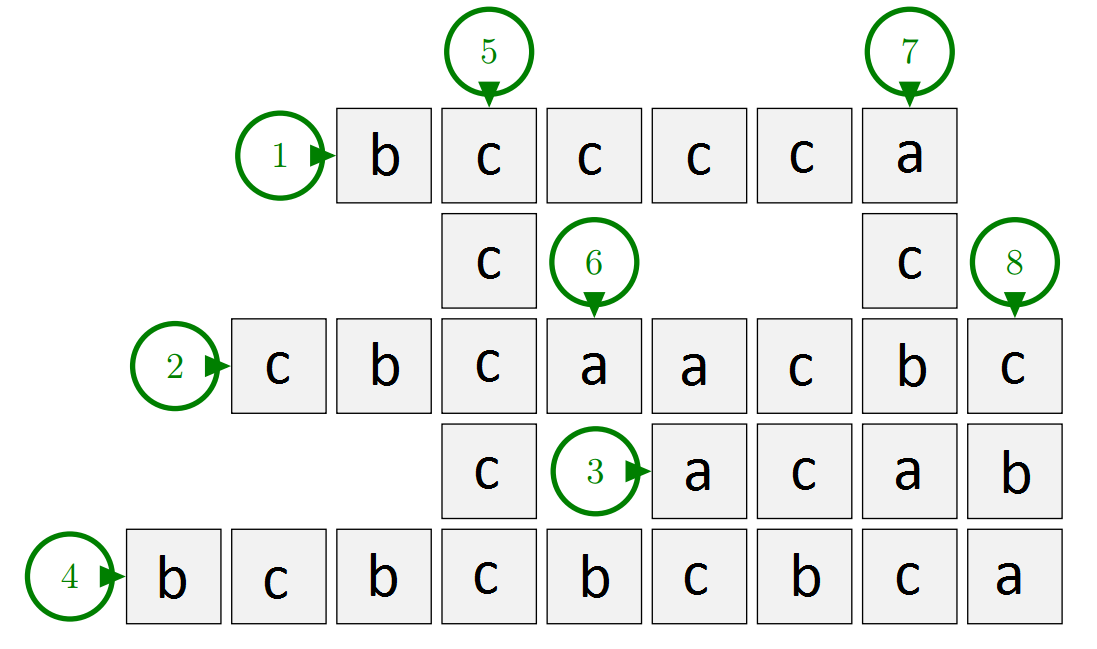
\includegraphics[scale=0.4]{crossword.png}
\end{figure}



\section*{Aufgabe 7.6}
\begin{center}
\textbf{Vom süßen Brei (1815)}

\textit{\footnotesize{aus: Brüder Grimm. Kinder- und Haus-Märchen Band 2, Große Ausgabe.}}
\end{center}
\begin{flushleft}\small
Es war einmal ein armes, frommes Mädchen, das lebte mit seiner Mutter allein und sie hatten nichts mehr zu essen. Da ging das Kind hinaus in den Wald und begegnete ihm darin eine alte Frau, die wußte seinen Jammer schon und schenkte ihm ein Töpfchen, zu dem sollt' es sagen: "`Töpfchen koch!"' so kochte es guten, süßen Hirschenbrei, und wenn es sagte: "`Töpfchen steh,"' so hörte es wieder auf zu kochen. Das Mädchen brachte den Topf seiner Mutter heim und nun waren sie ihrer Armuth und ihres Hungers ledig und aßen süßen Brei, so oft sie wollten. Auf eine Zeit war das Mädchen ausgegangen, da sprach die Mutter: "`Töpfchen koch!"' da kocht es und sie ißt sich satt; nun will sie, daß das Töpfchen wieder aufhören soll, aber sie weiß das Wort nicht. Also kocht es fort und der Brei steigt über den Rand heraus, und kocht immer zu, die Küche und das ganze Haus voll, und das zweite Haus und dann die Straße, als wollt’s die ganze Welt satt machen, und ist die größte Noth und kein Mensch weiß sich da zu helfen. Endlich, wie nur noch ein einziges Haus übrig ist, da kommt das Kind heim und spricht nur: "`Töpfchen steh!"' da steht es und hört auf zu kochen, und wenn sie wieder in die Stadt wollten, haben sie sich durchessen müssen.
\end{flushleft}

\subsection*{Inhalt}
Der Inhalt ist somit geklärt: Ein Mädchen bekommt einen kleinen Topf, dieser kocht für sie unendlich viel Brei bis sie ihn stoppt. Das führt natürlich zur Katastrophe, der mit Brei gefüllten Stadt. Die Katastrophe wird jedoch humorvoll gelöst: Das Töpfchen wird gestoppt und es passiert nichts weiter Schlimmes, als dass nun die Bewohner der Stadt sich durch den Brei essen müssen, um zurück zu ihren Häusern zu gelangen.

\subsection*{Beziehung Märchen - Erfindung}
Die Beziehung zwischen Märchen und der "`sehr vertrauten "`Erfindung"' von Stephen Cole Kleene"' ist ebenfalls simpel: 
Der Kleene-Stern funktioniert ein wenig wie das Töpfchen. Das Töpfchen produziert immer weiter Brei, während der Stern immer weiter Zeichen akzeptiert bzw. generiert (je nach Anwendungs- bzw. Interpretationskontext). 

\subsection*{Rolle von Kleene}
Die Frage, welche Rolle Kleene in diesem Märchen einnehmen würde, ist etwas komplizierter zu klären. In dem Märchen gibt es prinzipiell vier Rollen: Das Mädchen, die Mutter, die alte Frau und das Töpfchen. 
\begin{itemize}
	\item Da wir bereits klärten, dass das Töpfchen dem Kleene-Stern entspricht, liegen zwei Personen für Kleene nahe: Das Mädchen oder die alte Frau. Die Mutter ist auszuschließen, da diese die Katastrophe herbeiführt - Kleenes Erfindung ist aber eher nütz- als hinderlich.
  \item Die alte Frau hat das Töpfchen zuerst und gibt es dem Mädchen. Sie stellt viele Fragen: Woher ist das Töpfchen, warum ist sie im Wald, ...? Die Antwort ist: Die alte Frau steht für etwas, das vor dem Mädchen (und vielleicht dem Töpfchen?) existierte. Im übertragenen Sinne können wir sie als Symbol für die Mathematik, die Informatik oder auch ganz konkret die Automatentheorie oder Rekursionstheorie sehen. 
  \item Das Mädchen bekommt das Töpfchen von der alten Frau. Es also ein Werkzeug, um ein Problem zu lösen (in der Geschichte der Hunger und die Armut). Dieses Werkzeug macht sie sich zu nutzen und stellt es auch anderen zu Verfügung, die jedoch erst lernen müssen, es zu verwenden. 
\end{itemize}

Kleene handelt wie das Mädchen: Er erhält bzw. erfindet ein Werkzeug um ein Problem zu lösen. Das Werkzeug ist der Kleene-Stern, bzw. die mathematische Idee, die er repräsentiert. Kleene bekommt die Idee aus der Mathematik, indem er versucht das Problem zu lösen, Schleifen in Automaten sinnvoll beschreiben zu können. Wie das Mädchen, das in den Wald ging, um den Hunger zu stillen, sucht Kleene in der Mathematik nach dieser Lösung und bekommt sie. Wie das Mädchen bringt er das Werkzeug zu anderen, die es ebenfalls gern nutzen möchten - den Umgang aber erst lernen müssen. Kleenes Rolle wäre somit klar die des Mädchens.



\end{document}
